\ \\ [-3mm]
   {\hautab{1.5}
   {\setlength{\tabcolsep}{1mm}
   \begin{cltableau}{1\linewidth}{7}
      \hline
      & 12 & 40 & 248 & 3 019 & 1 002 & 1 003 \\
      \hline
      & & & \large\textpmhg{\Hhundred\Hhundred} & \multirow{2}{*}{\large\textpmhg{\Hthousand\Hthousand\Hthousand}} & \multirow{3}{*}{\large\textpmhg{\Hthousand\Hone\Hone}} & \multirow{3}{*}{\large\textpmhg{\Hthousand\Hone\Hone\Hone}} \\
      Égyptien & \large\textpmhg{\Hten\Hone\Hone} & \large\textpmhg{\Hten\Hten\Hten\Hten} & \large\textpmhg{\Hten\Hten\Hten\Hten} & & & \\
      & & & \large\textpmhg{\Hone\Hone\Hone\Hone\Hone\Hone\Hone\Hone} & \large\textpmhg{\Hten\Hone\Hone\Hone\Hone\Hone\Hone\Hone\Hone\Hone} & & \\
      \hline
      Romain & \cRm{12} & \cRm{40} & \cRm{248} & \cRm{3019} & \cRm{1002} & \cRm{1003} \\
      \hline
      & 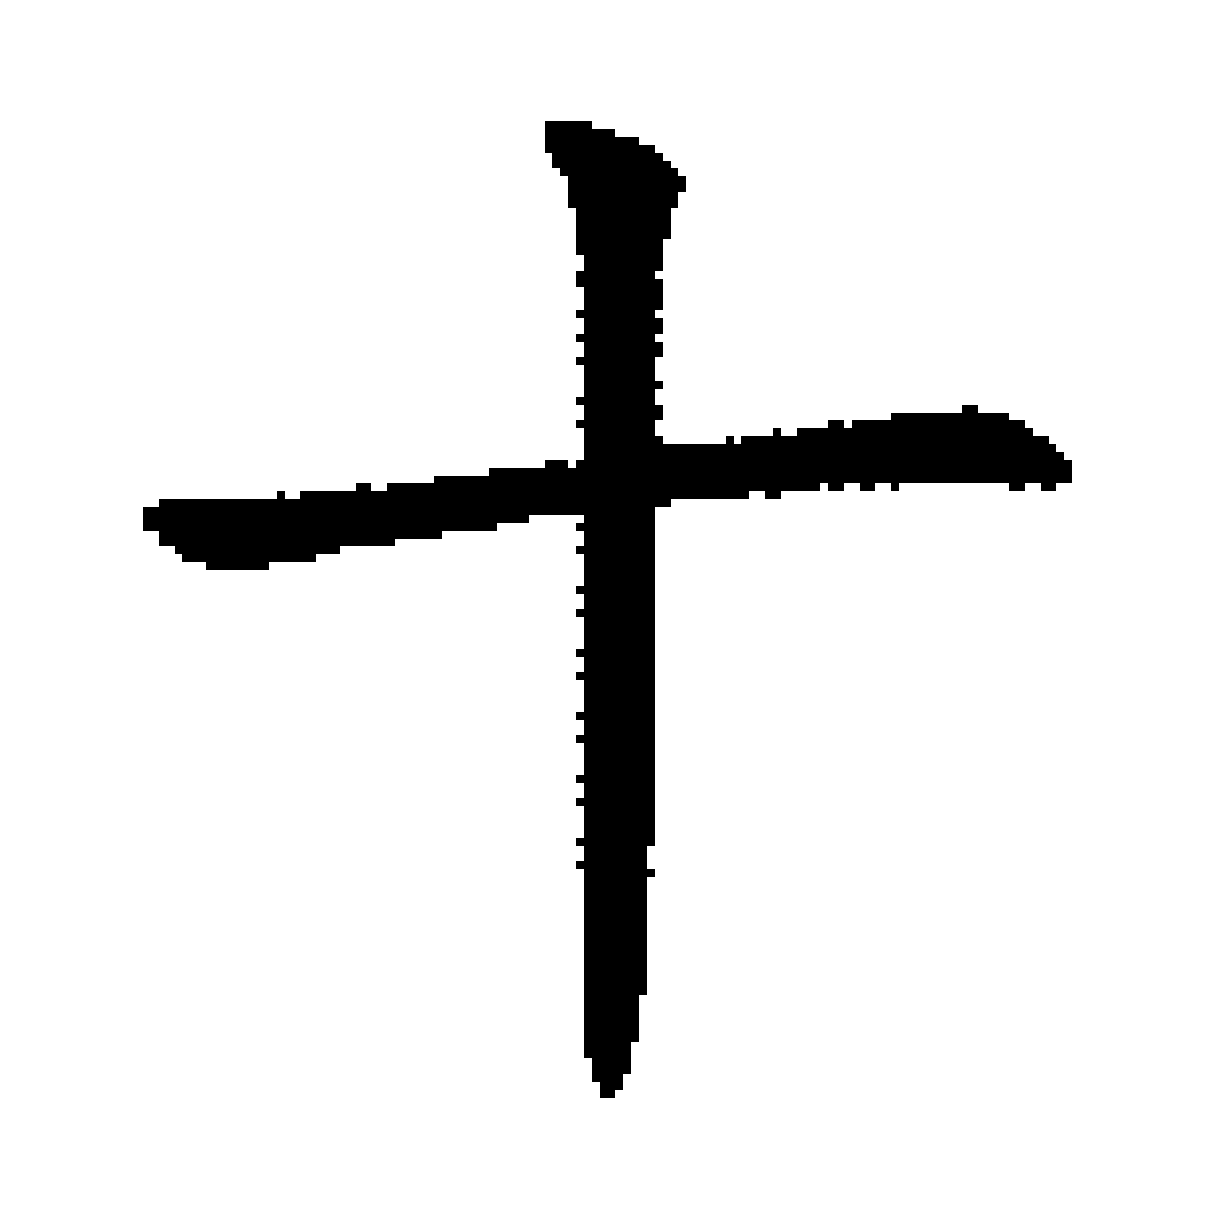
\includegraphics[width=5mm]{Nombres_et_calculs/Images/N1_chinois10} & 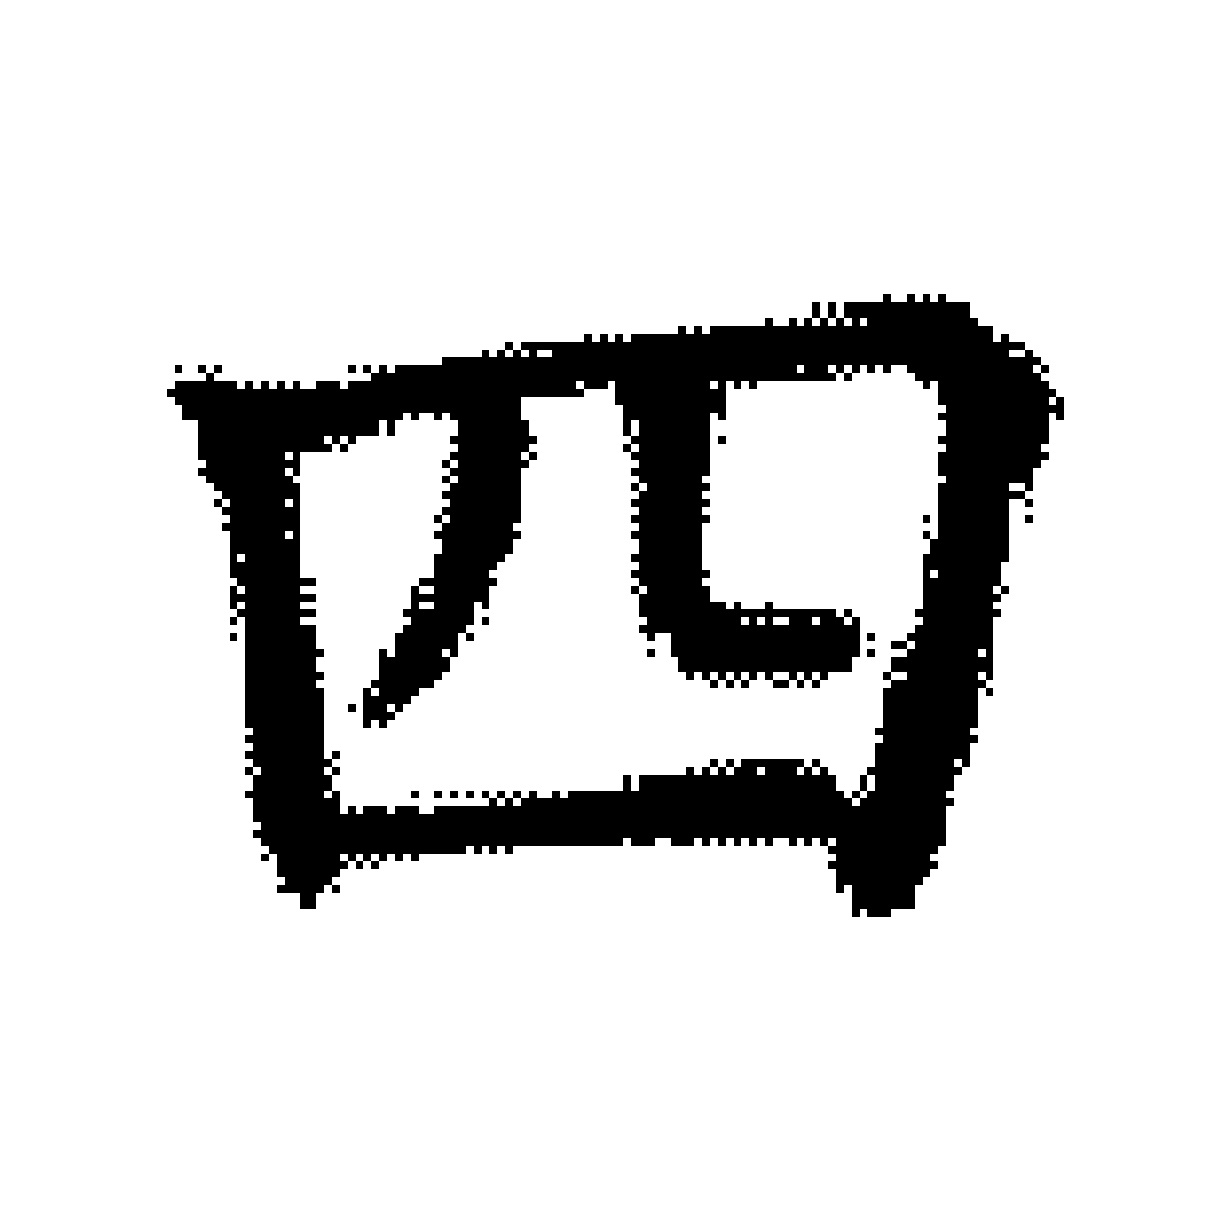
\includegraphics[width=5mm]{Nombres_et_calculs/Images/N1_chinois4} & 
\includegraphics[width=5mm]{Nombres_et_calculs/Images/N1_chinois2} & 
\includegraphics[width=5mm]{Nombres_et_calculs/Images/N1_chinois3} & 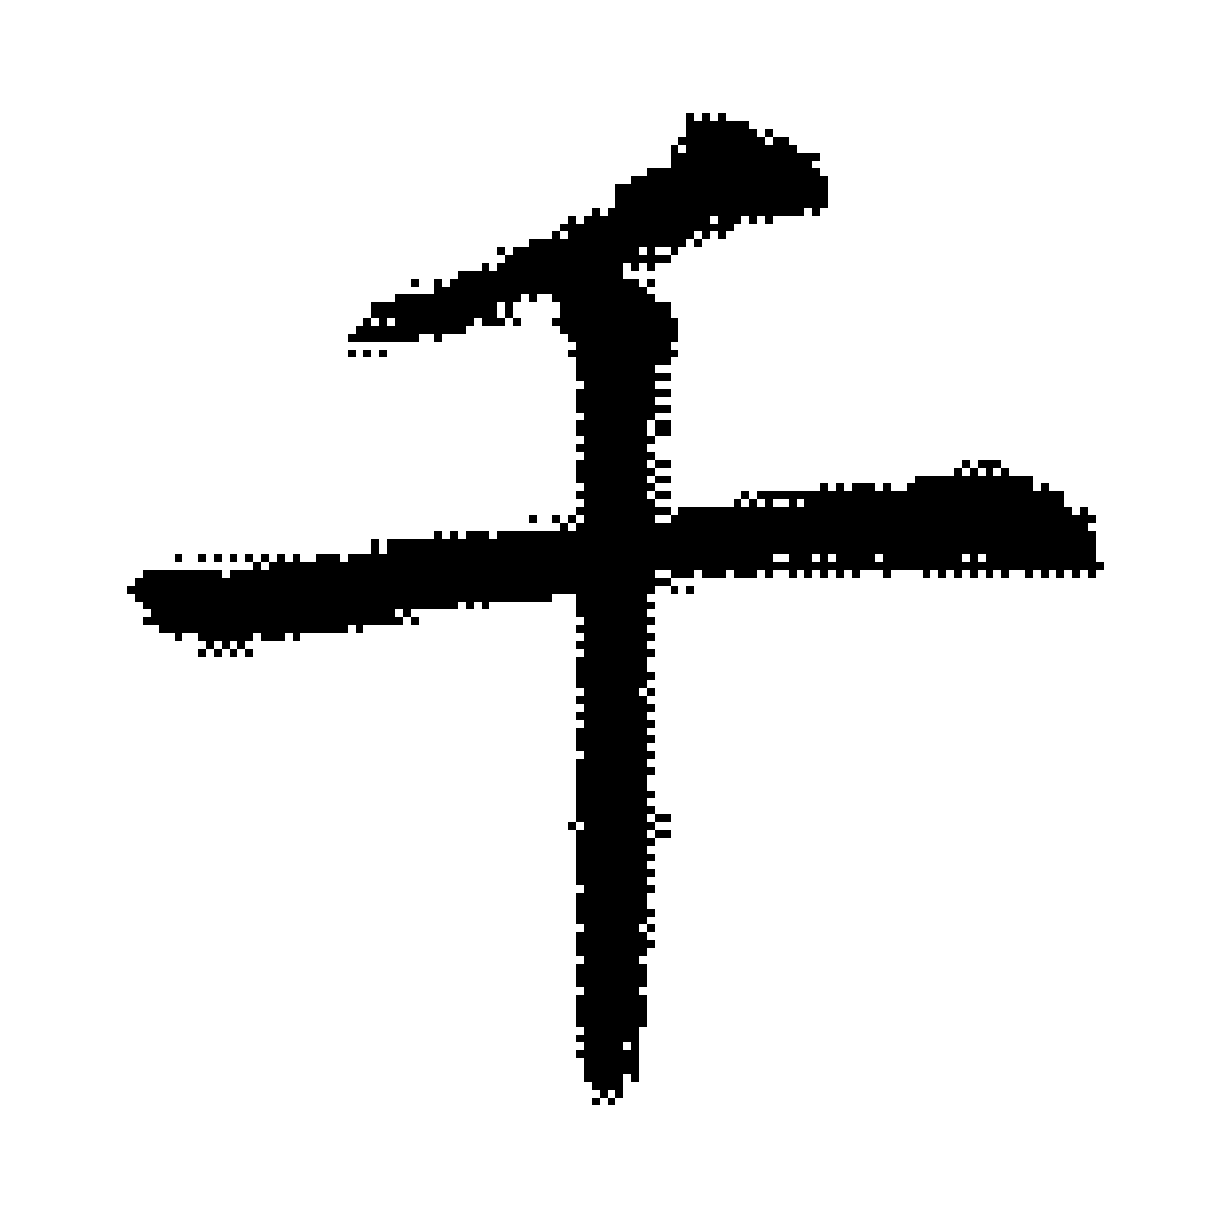
\includegraphics[width=5mm]{Nombres_et_calculs/Images/N1_chinois1000} & 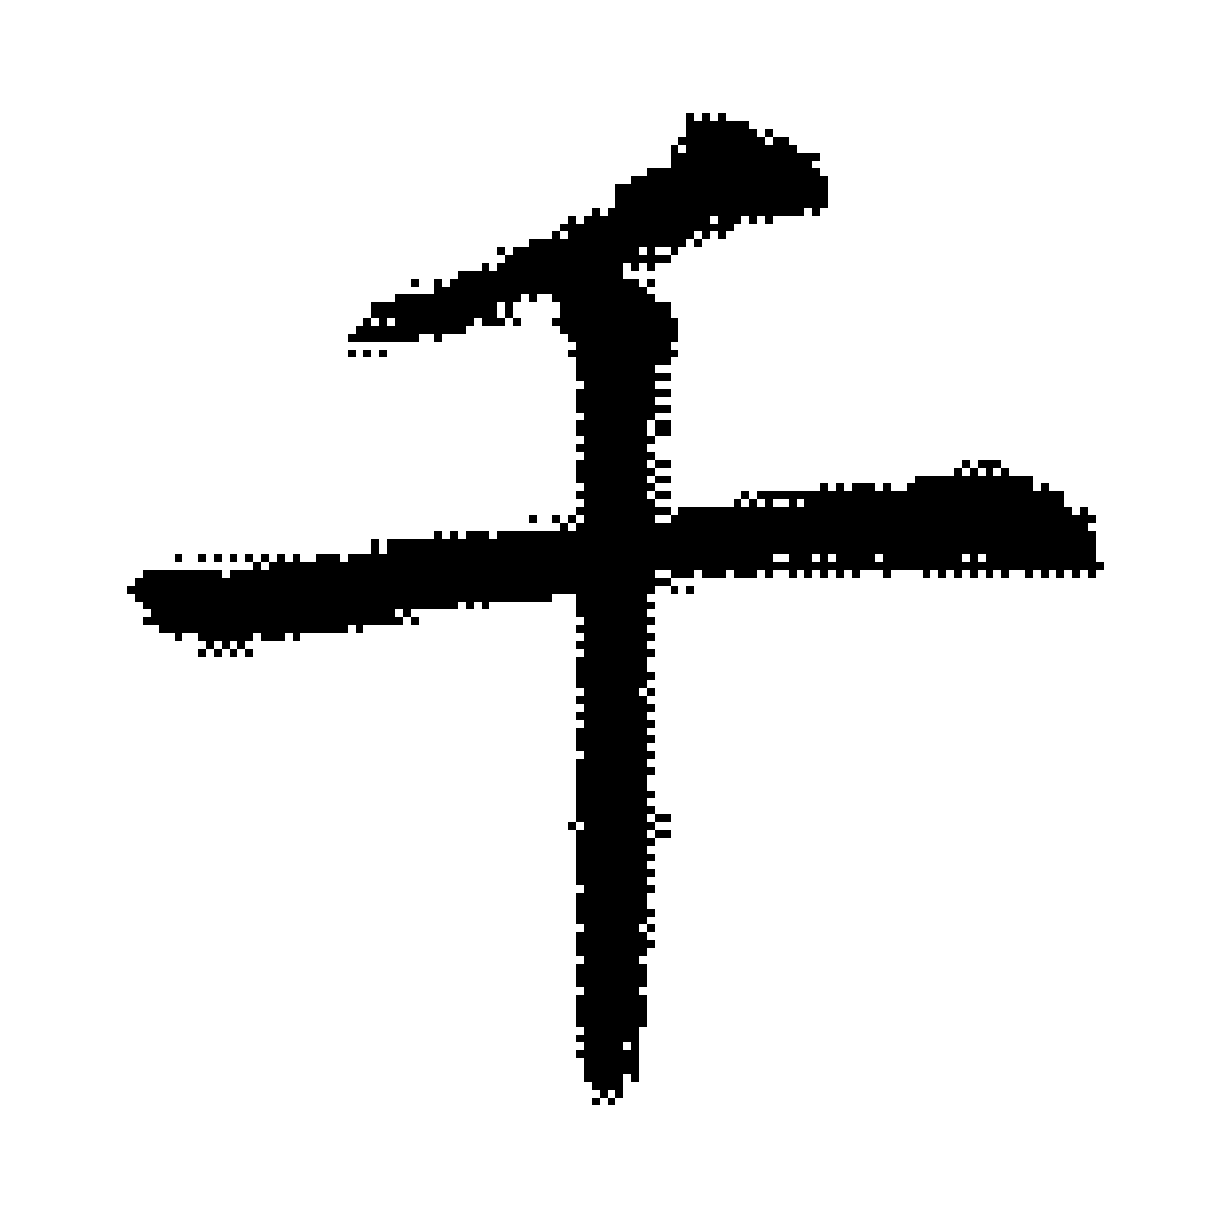
\includegraphics[width=5mm]{Nombres_et_calculs/Images/N1_chinois1000} \\
      & 
\includegraphics[width=5mm]{Nombres_et_calculs/Images/N1_chinois2} & 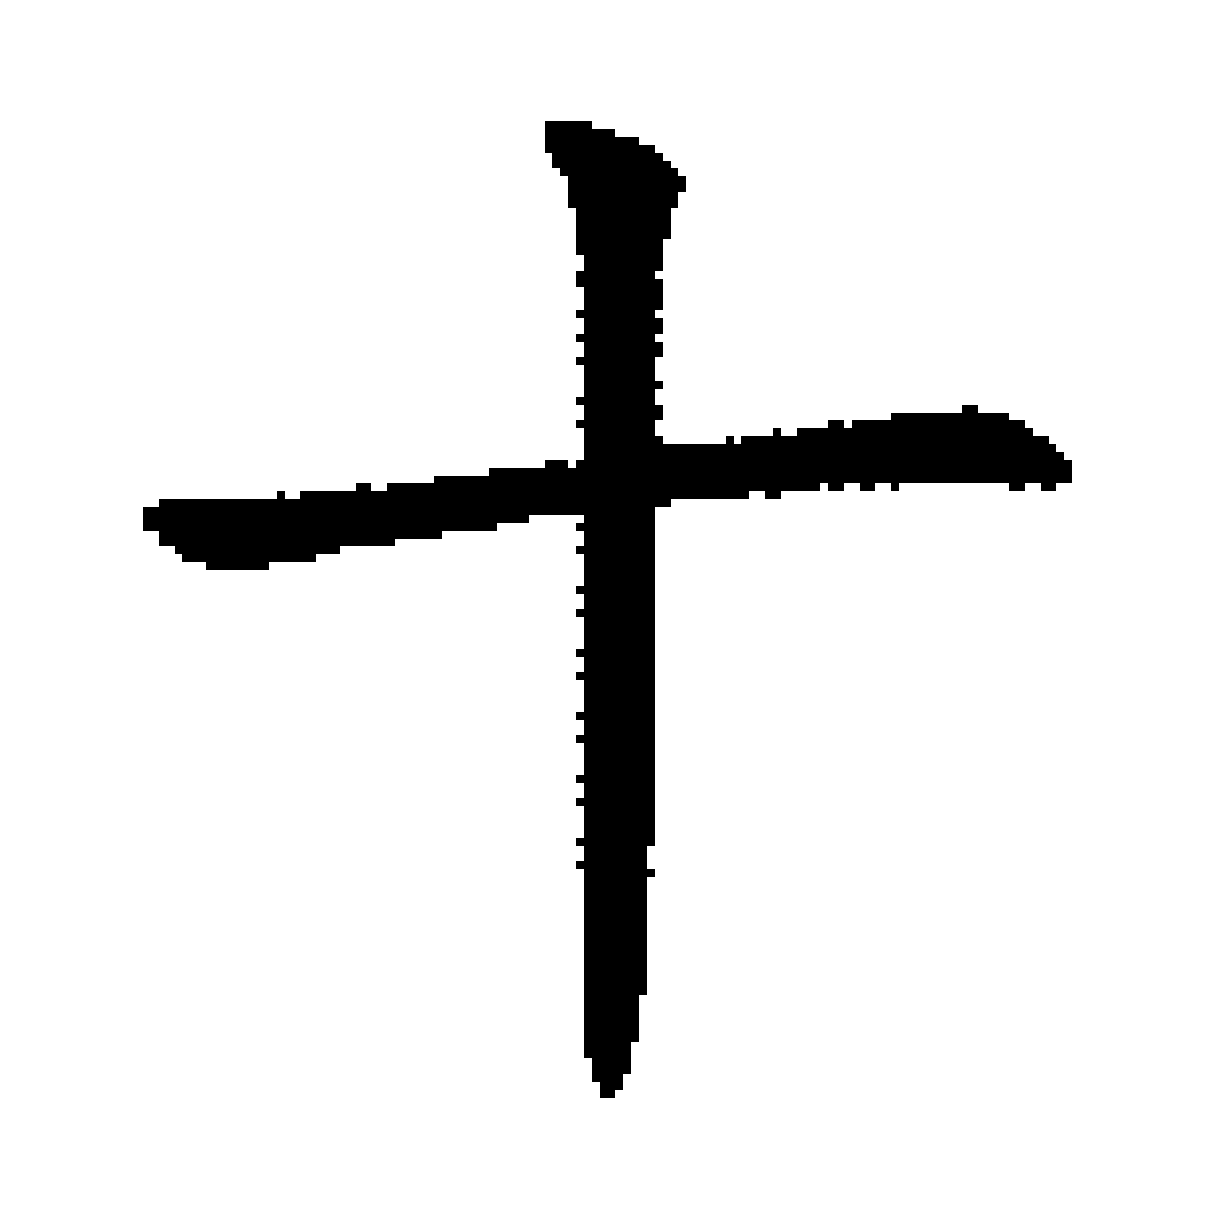
\includegraphics[width=5mm]{Nombres_et_calculs/Images/N1_chinois10} & 
\includegraphics[width=5mm]{Nombres_et_calculs/Images/N1_chinois100} & 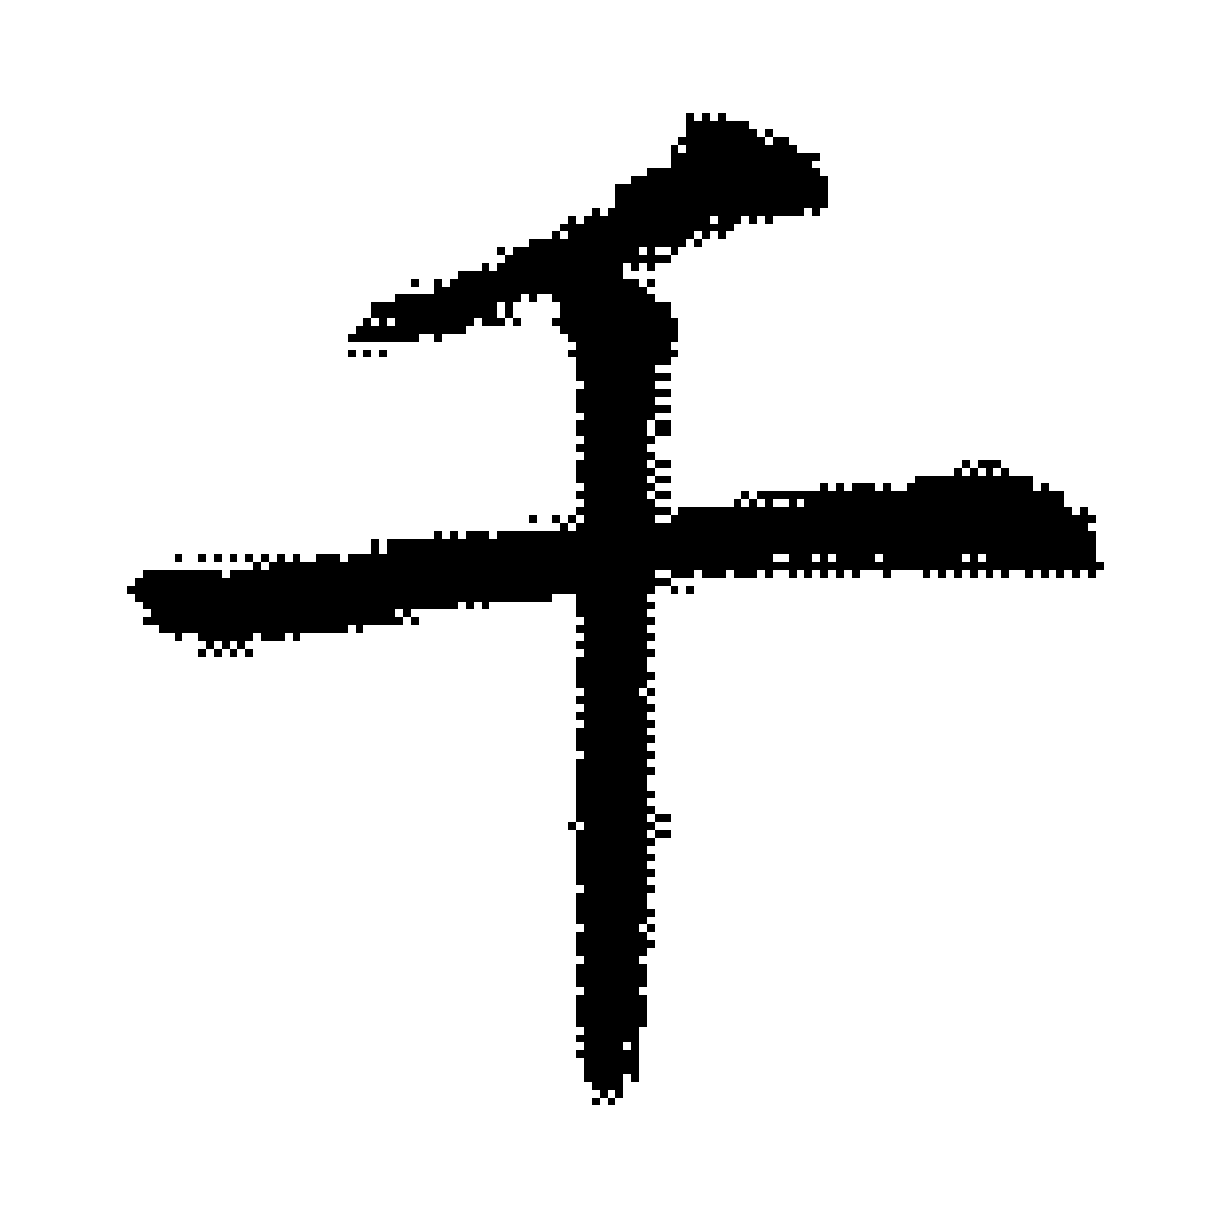
\includegraphics[width=5mm]{Nombres_et_calculs/Images/N1_chinois1000} & 
\includegraphics[width=5mm]{Nombres_et_calculs/Images/N1_chinois2} & 
\includegraphics[width=5mm]{Nombres_et_calculs/Images/N1_chinois3} \\
      Chinois & & & 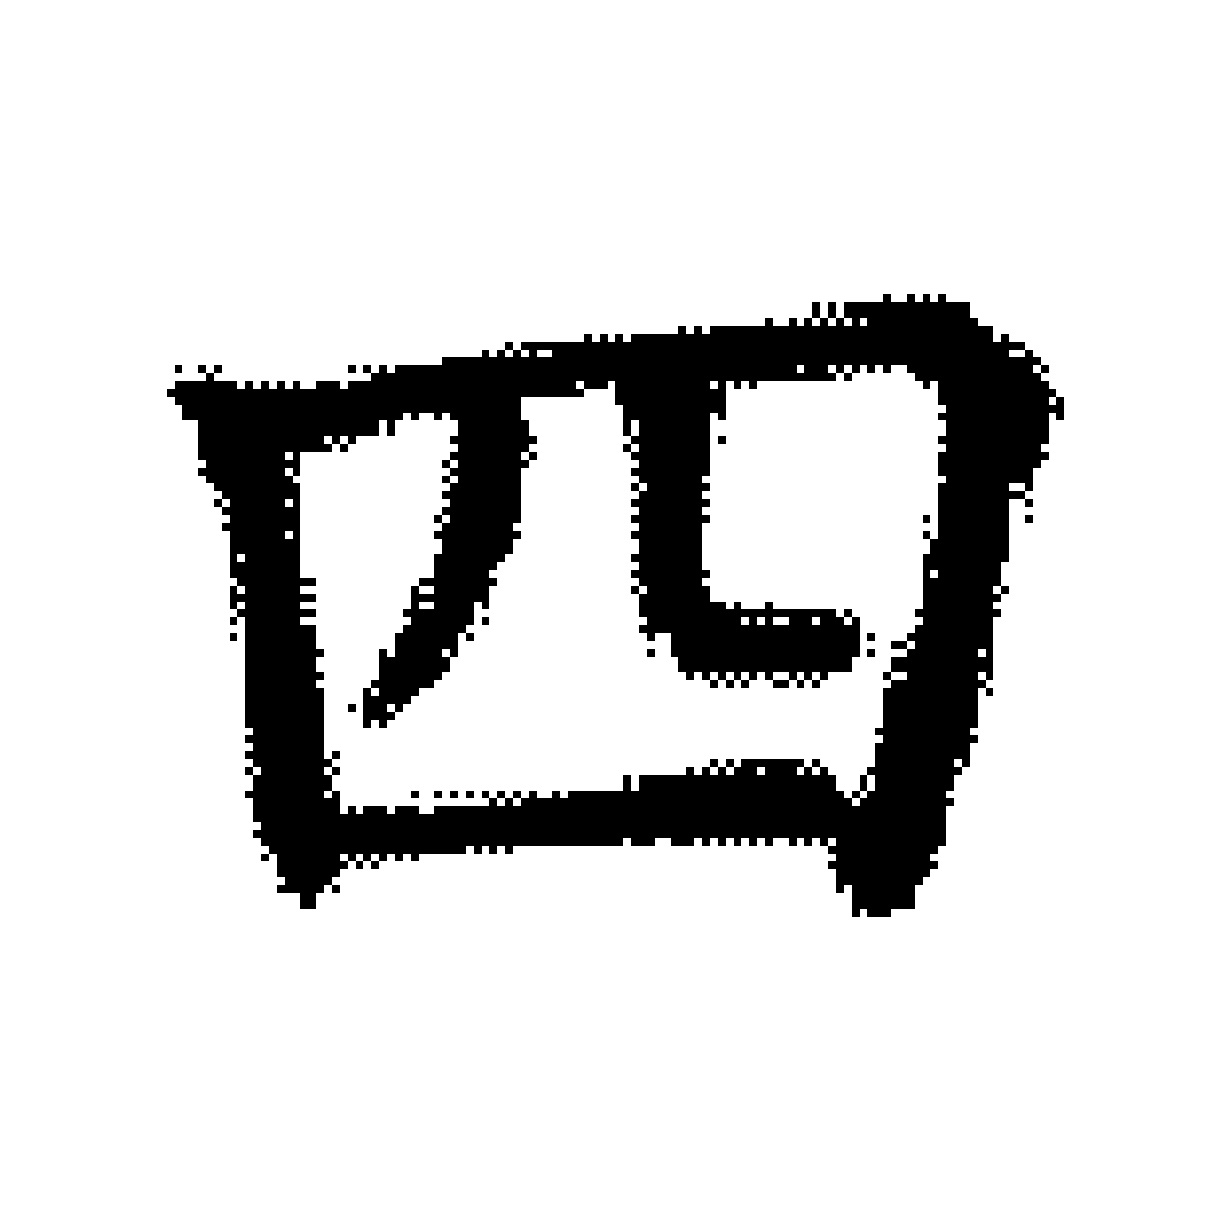
\includegraphics[width=5mm]{Nombres_et_calculs/Images/N1_chinois4} & 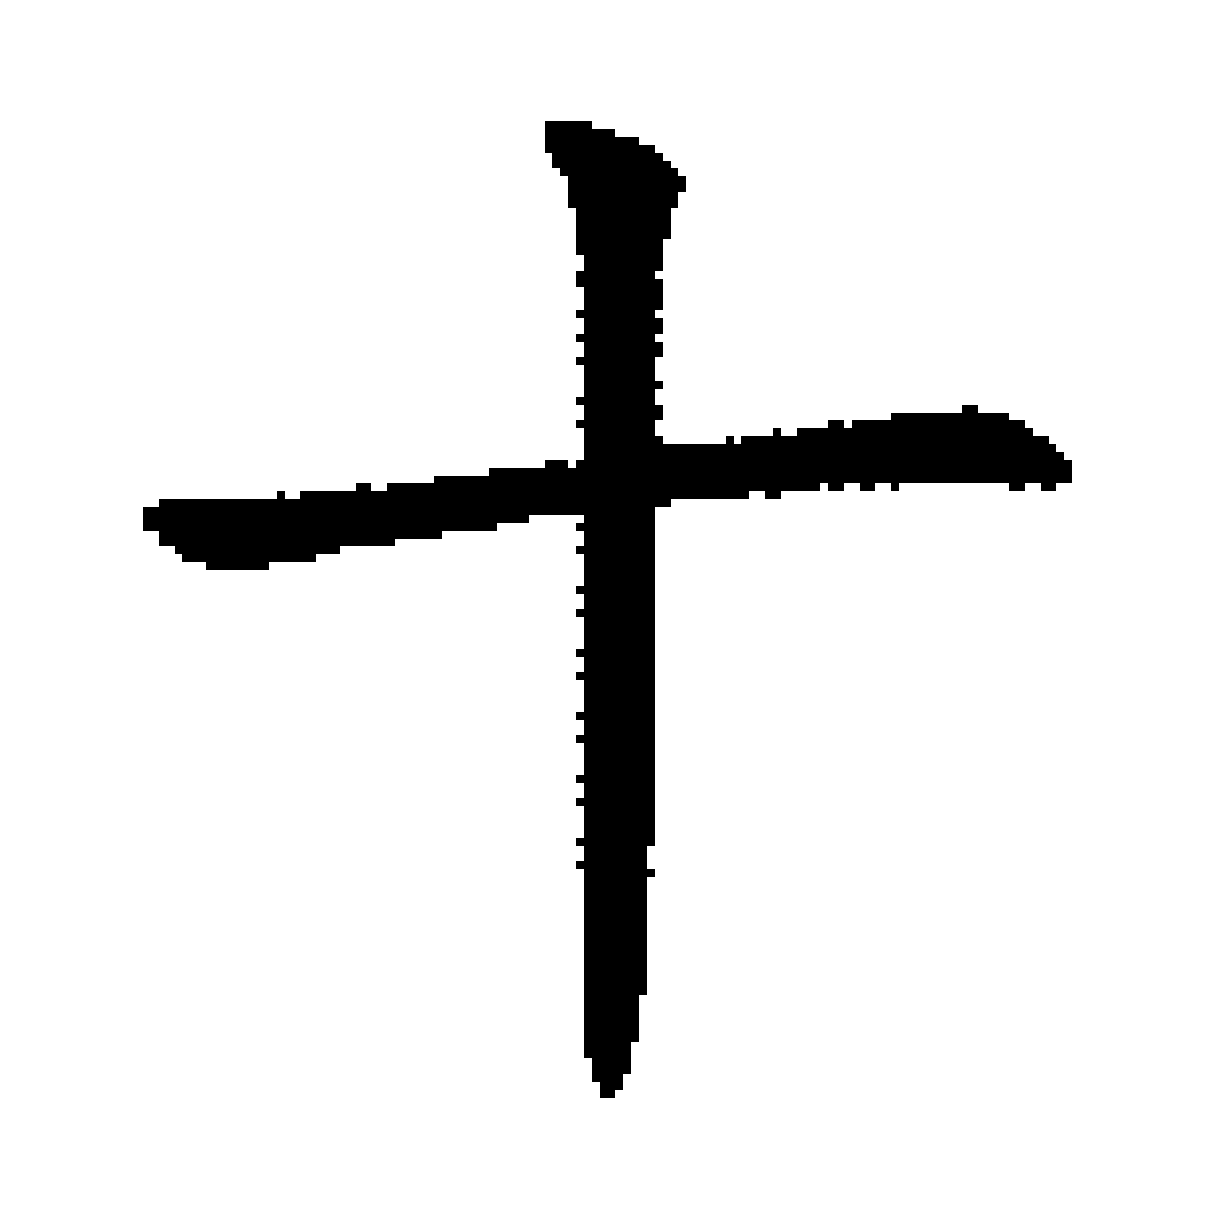
\includegraphics[width=5mm]{Nombres_et_calculs/Images/N1_chinois10} & & \\
      & & & 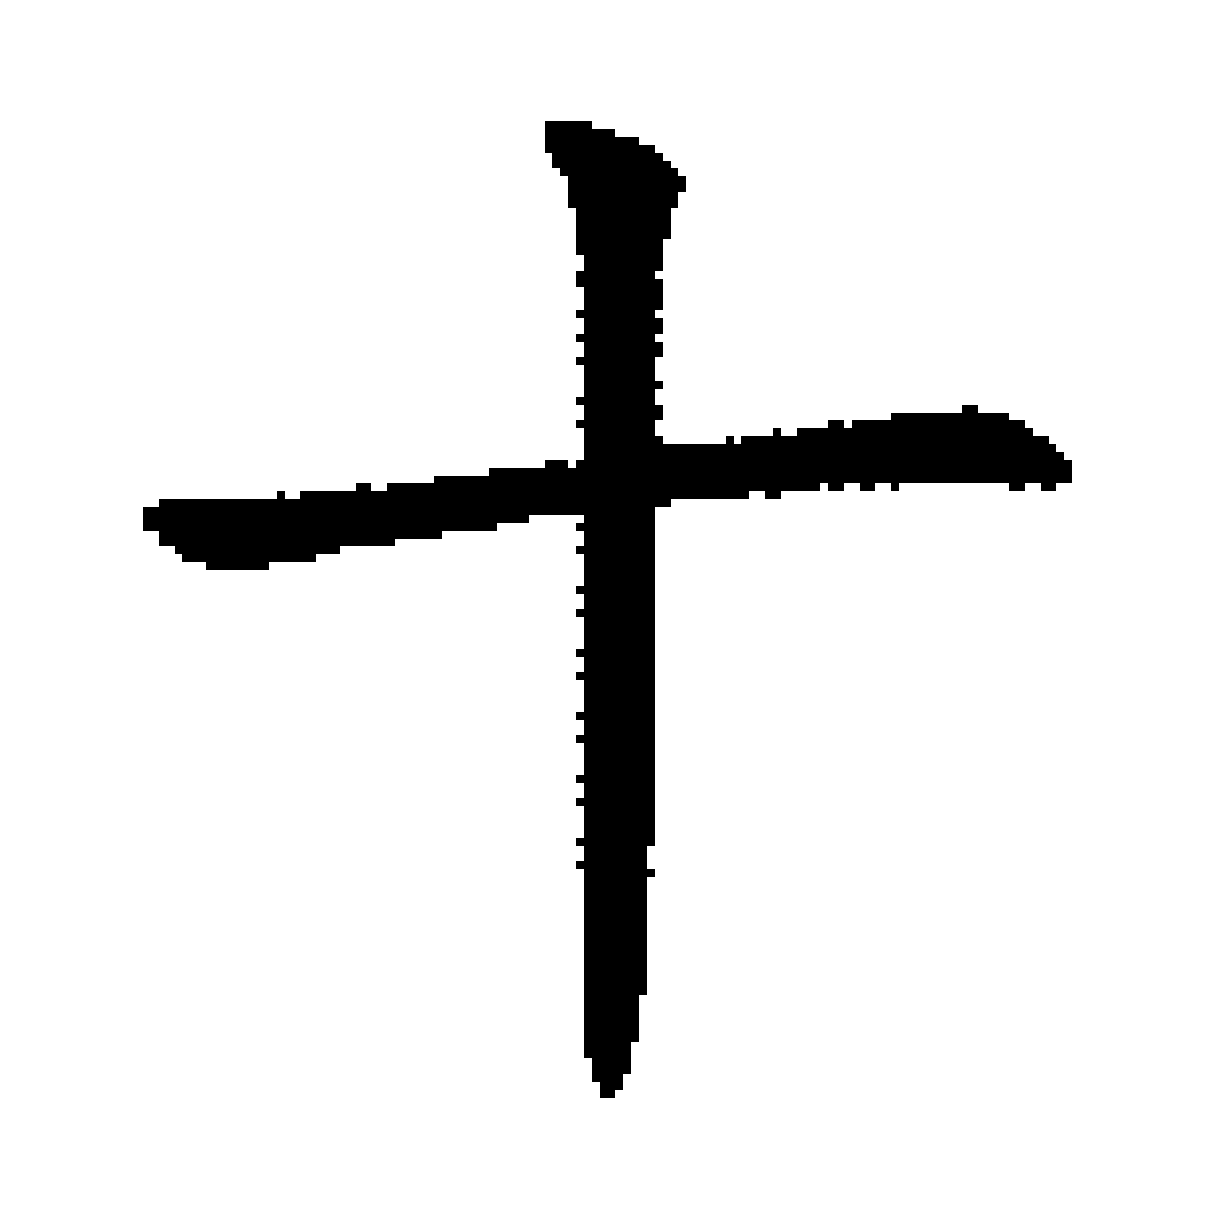
\includegraphics[width=5mm]{Nombres_et_calculs/Images/N1_chinois10}  & 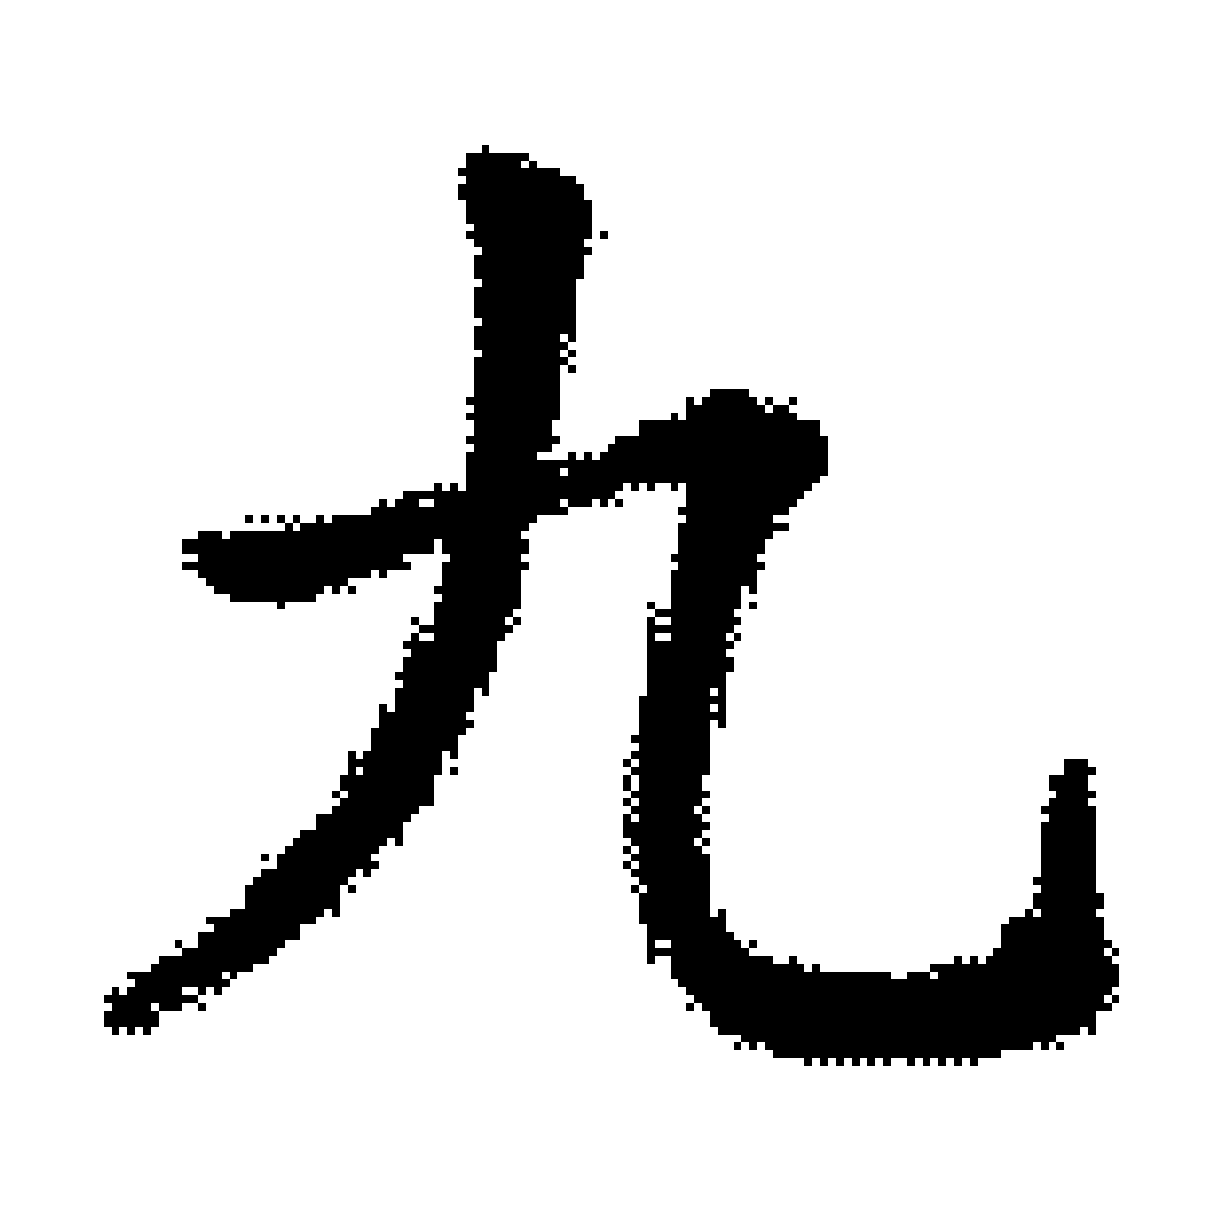
\includegraphics[width=5mm]{Nombres_et_calculs/Images/N1_chinois9} & & \\
      & & & 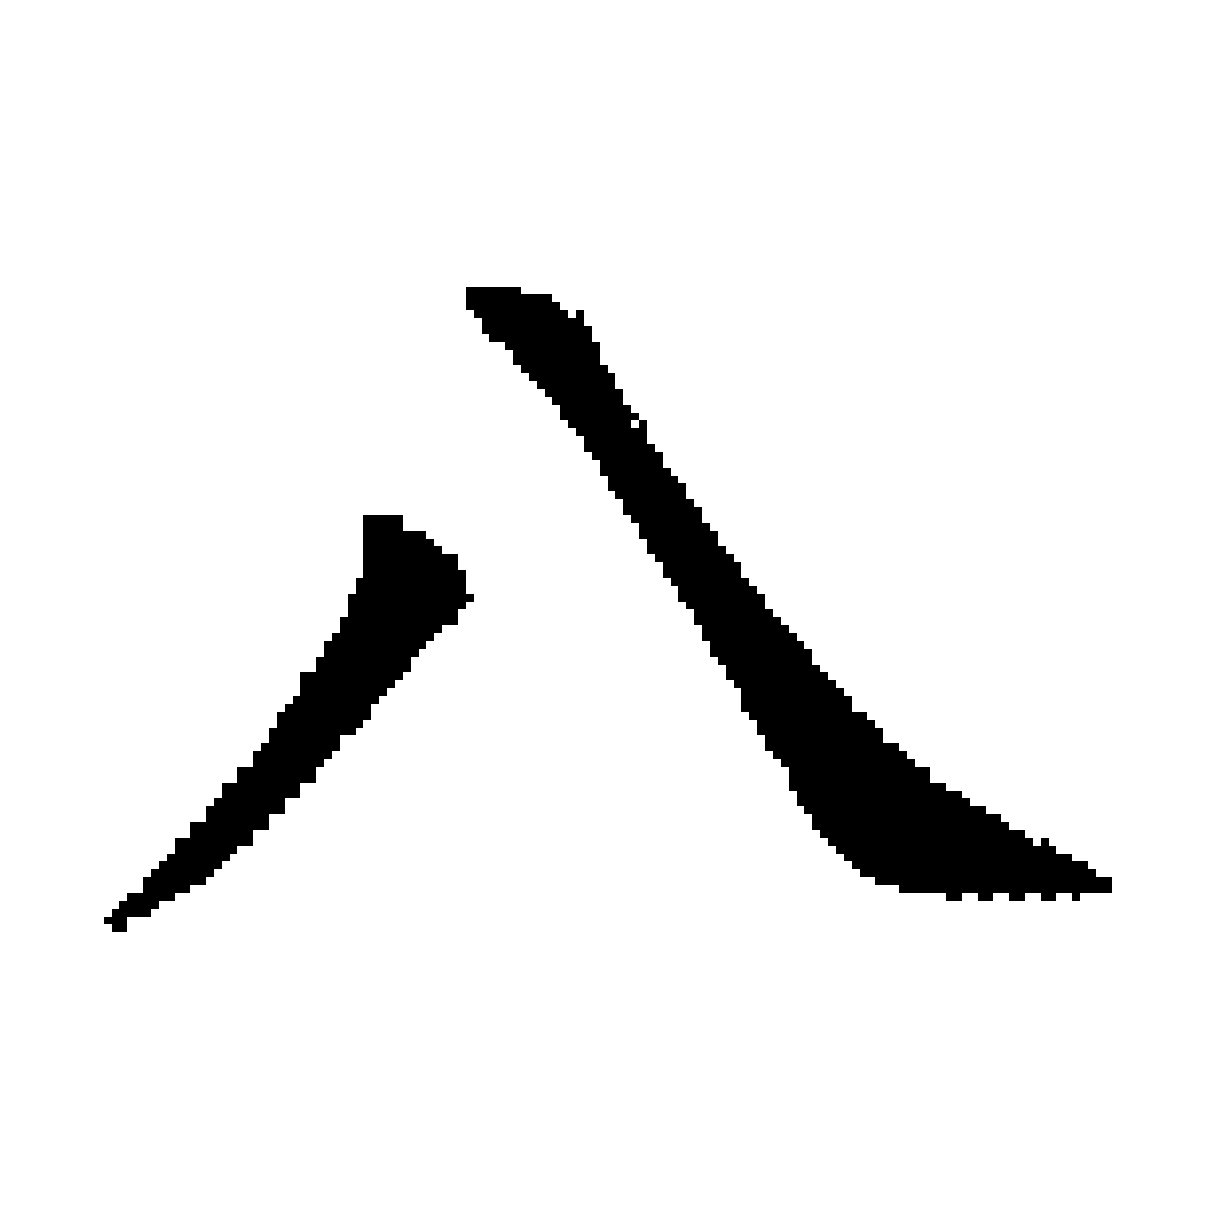
\includegraphics[width=5mm]{Nombres_et_calculs/Images/N1_chinois8} & & & \\
      \hline
         Maya & \large$\maya{12}$ & \large$\maya{40}$ & \large$\maya{248}$ & \large$\maya{3019}$ & \large$\maya{1002}$ & \large$\maya{1003}$ \\ [8mm]
      \hline
      Binaire & 1100 & 101000 & 11111000 & 10111100101 & 1111101010 & 1111101011 \\
      \hline
   \end{cltableau}}}
   \begin{remarque}
      la numération Maya n'utilisait pas strictement une base 20, il existait en effet une irrégularité où le passage de l'ordre 2 à l'ordre 3 nécessitait une multiplication par 18 au lieu de 20. Dans le cadre du CRPE, il est très probable que cette irrégularité ne soit pas prise en compte et c'est pour ce cas que le corrigé a été fait.
   \end{remarque}
